\NeedsTeXFormat{LaTeX2e}
\documentclass[a4paper,10pt,twoside,openright,DIV=15,BCOR25mm
%,draft
]{scrbook}
\KOMAoptions{DIV=last}


\pagestyle{headings}
\usepackage[ngerman]{babel}

\usepackage{subfigure}

%\usepackage[latin1]{inputenc}
%\usepackage[applemac]{inputenc} % Mac-Nutzer
\usepackage[utf8]{inputenc}
\usepackage[T1]{fontenc}
\renewcommand{\sfdefault}{phv}
\renewcommand{\rmdefault}{phv}
\renewcommand{\ttdefault}{pcr}
\usepackage{graphicx}
\usepackage{verbatim}
\usepackage{tabularx}
\usepackage{url}
\usepackage{color}
\usepackage{amssymb}
\usepackage{amsmath}
\usepackage{setspace}
\usepackage{listings}
\renewcommand{\lstlistingname}{Algorithm}% Listing -> Algorithm
\renewcommand{\lstlistlistingname}{List of \lstlistingname s}% List of Listings -> List of Algorithms
\usepackage{todonotes}
\usepackage{hyperref}
\usepackage{array}
%\usepackage[table]{xcolor}
\usepackage{colortbl}
\usepackage{booktabs}
\usepackage{float}
%\usepackage{svg}


\lstset{language=VHDL,
  showstringspaces=false,
  frame=single,
  numbers=left,
  basicstyle=\ttfamily,
  numberstyle=\tiny}

% hier Namen etc. einsetzen
\newcommand{\fullname}{Heiko~Foschum}
\newcommand{\email}{heiko.foschum@gmx.de}
\newcommand{\titel}{Konzeption und Realisierung  einer Plattform zur Unterstützung  von therapeutischen Übungen  und Aufgaben}
\newcommand{\jahr}{2016}
\newcommand{\matnr}{856456}
\newcommand{\gutachterA}{Prof. Dr. Manfred Reichert}
\newcommand{\gutachterB}{Dr. Rüdiger Pryss}
\newcommand{\betreuer}{Marc Schickler}
% hier richtige Fakultät auswählen
\newcommand{\fakultaet}{Ingenieurwissenschaften\\und Informatik}
%\newcommand{\fakultaet}{Mathematik und\\Wirtschaftswissenschaften}
%\newcommand{\fakultaet}{Naturwissenschaften}
%\newcommand{\fakultaet}{Medizin}
% nun noch unten das Institut einsetzen
\newcommand{\institut}{Institut für Datenbanken und Informationssysteme}

%color in tables
\usepackage{colortbl}
\definecolor{Gray}{rgb}{0.80784, 0.86667, 0.90196} %dunkelblau
\definecolor{Lightgray}{rgb}{0.9176, 0.95, 0.95686} %hellblau
\definecolor{Akzent}{rgb}{0.6627, 0.63529, 0.55294} %akzentfarbe
\setlength{\arrayrulewidth}{0.1pt}

\clubpenalty 10000
\widowpenalty 10000

\setlength{\parindent}{0pt}
\setlength{\parskip}{1.4ex plus 0.35ex minus 0.3ex}

% Tiefe, bis zu der Überschriften in das Inhaltsverzeichnis kommen
\setcounter{tocdepth}{3}

\pdfinfo{
  /Author (\fullname)
  /Title (\titel)
  /Producer     (pdfeTex 3.14159-1.30.6-2.2)
  /Keywords ()
}

\usepackage{hyperref}
\hypersetup{
pdftitle=\titel,
pdfauthor=\fullname,
pdfsubject={Masterarbeit},
pdfproducer={pdfeTex 3.14159-1.30.6-2.2},
colorlinks=false,
pdfborder=0 0 0	% keine Box um die Links!
}

%Trennungsregeln
\hyphenation{Sil-ben-trenn-ung}
\hyphenation{Sprung-se-quenz-en}
\hyphenation{Sprung-se-quenz}
\hyphenation{Ka-nal-mo-del}
\hyphenation{Ka-nal-mo-dels}
\hyphenation{Bit-Sen-de-dau-er}
\hyphenation{Im-ple-men-tie-rung}
\hyphenation{VHDL-Im-ple-men-tie-rung}
\hyphenation{Sen-de-dau-er}
\hyphenation{FH-FSK-Mo-du-la-ti-on}

\begin{document}
\frontmatter


%Einstellung der Farbe von Tabellen
%\rowcolors{1}{green}{pink}
% Titelseite
\thispagestyle{empty}
\begin{addmargin*}[4mm]{-10mm}


\includegraphics[height=1.8cm]{images/unilogo_bild}
\hfill

\includegraphics[height=1.8cm]{images/unilogo_wort}\\[1em]

{\footnotesize
{\bfseries Universität Ulm} \textbar ~89069 Ulm \textbar ~Germany
\hspace*{50mm}\parbox[t]{65mm}{\bfseries Fakultät für\\
\fakultaet\\
% TODO hier Institut anpassen
\mdseries \institut}\\[2cm]

\parbox{140mm}{\bfseries \huge \titel}\\[0.5em]
{\footnotesize Masterarbeit}\\[3em]

{\footnotesize \bfseries Vorgelegt von:}\\
{\footnotesize \fullname\\\email}\\[2em]
%{\footnotesize \bfseries Bearbeitet mit:}\\                     
%{\footnotesize\bearbeitetMit\\\bearbeitetMitEmail}\\[2em]
{\footnotesize \bfseries Gutachter:}\\ 
{\footnotesize\gutachterA\\
\gutachterB}\\[2em]
{\footnotesize \bfseries Betreuer:}\\ 
{\footnotesize\betreuer}\\\\
{\footnotesize\jahr}
}
\end{addmargin*}


% Impressum
\clearpage
\thispagestyle{empty}
{ \small
  \flushleft
  Fassung \today \\\vfill
  \copyright~\jahr~\fullname\\[0.5em]
% Falls keine Lizenz gewünscht wird bitte den folgenden Text entfernen.
% Die Lizenz erlaubt es zu nichtkommerziellen Zwecken die Arbeit zu
% vervielfältigen und Kopien zu machen. Dabei muss aber immer der Autor
% angegeben werden. Eine kommerzielle Verwertung ist für den Autor
% weiter möglich.
%This work is licensed under the Creative Commons Attribution-NonCommercial-ShareAlike 3.0 License. To view a copy of this license, visit http://creativecommons.org/licenses/by-nc-sa/3.0/de/ or send a letter to Creative Commons, 543 Howard Street, 5th Floor, San Francisco, California, 94105, USA. \\
  Satz: PDF-\LaTeXe
}


% ab hier Zeilenabstand 1,4 fach 10pt/14pt
\setstretch{1.4}

\tableofcontents

\mainmatter
\chapter{Einleitung}
Bei der Betreuung von Patienten durch einen Therapeuten, ob nun in der Psycho-, Physiotherapie oder sogar in der Diätassistenz, sind neben der eigentlichen \textbf{Therapie / Behandlung} durch den Therapeuten - Übungen und Fragebögen für Zuhause fast immer Bestandteil der Behandlung. Wie in Abbildung \ref{TherapieAblauf} aufgezeigt werden die Aufgaben in der Sitzung besprochen und sollen dann von dem Patienten selbstständig und ohne Betreuung bearbeitet werden.

\begin{figure}[H]
	\centering
	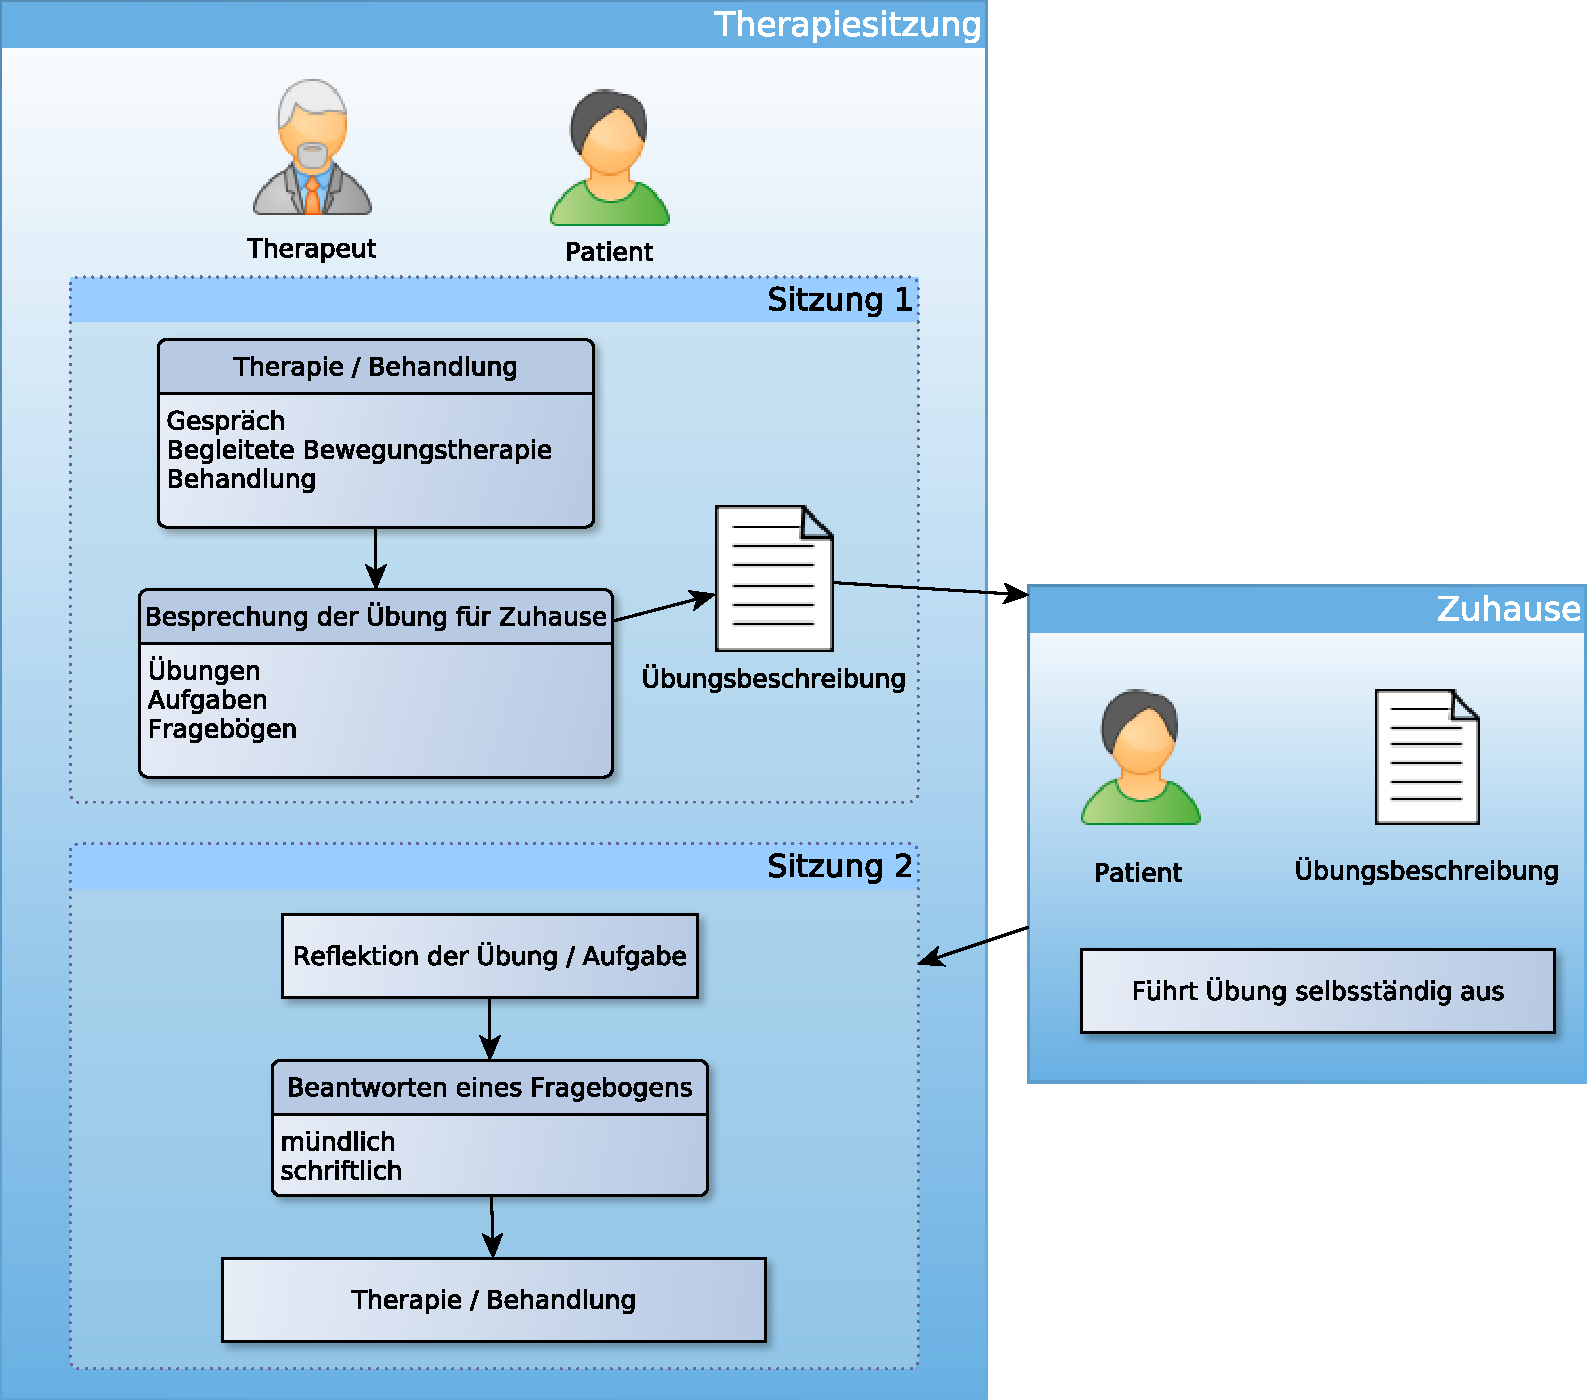
\includegraphics[scale=0.55]{images/TherapieAblauf}
	\caption[Grundlegender Ablauf einer Therapie]{Grundlegender Ablauf einer Therapie}
	\label{TherapieAblauf}
\end{figure}

Diese Aufgaben sind wichtiger Bestandteil für den Behandlungserfolg \cite{SL05}. Sie helfen beim Transfer der Therapie in den Alltag. Jedoch ist eins der größten Probleme bei dieser Vorgehensweise, dass die Aufgaben oft gar nicht oder nur unvollständig erledigt werden \cite{FF01}.

Bisher wurden dieses Aufgaben auf einen Blatt Papier festgehalten und der Patient war selbst dafür verantwortlich diese in seinen Tagesablauf einzuplanen. Die einzige Vorgabe war es, die Aufgabe(n) bis zum nächsten Termin x mal zu machen. Der Therapeut gab im besten Fall lediglich eine Empfehlung wann die Aufgabe zu erledigen ist, nicht jedoch einen genauen Plan an den sich der Patient halten konnte.
\section{Ziel der Arbeit}

Im Zuge dieser Arbeit wurde das Konzept einer Plattform entwickelt und umgesetzt, welches auf der einen Seite dem Patienten hilft sein Aufgabe zu erledigen. Auf der anderen Seite aber auch dem Therapeuten Daten und Feedback zu den Übungen liefert, wodurch dieser die Möglichkeit hat den Behandlungserfolg zu steigern.

Auf Grundlage aktueller Software wurde so eine Plattform implementiert, die es dem Therapeuten erlaubt seine Patienten innerhalb einer Webanwendung zu verwalten. Er hat die Möglichkeit, Therapieaufgaben und Fragebögen zu gestalten und diese dem jeweiligen Patienten zuzuordnen.

Anhand einer App wird der Patient sobald das Zeitintervall angefangen hat, daran erinnert seine Aufgabe zu erledigen und zeigt die Aufgabenbeschreibung an. Am Ende des definierten Zeitintervalls hat der Patient die Möglichkeit den zugeordneten Fragebogen auszufüllen. Welcher nach Beendigung wiederum direkt vom Therapeuten eingesehen werden kann.

Ziel ist es vor allem, das die Aufgaben vollständig und vor allem immer erledigt werden. Aber auch die erzeugte Resonanz und Daten soll zum Therapieerfolg beitragen. Hierdurch können die therapeutischen Aufgaben/Übungen verbessert werden und auf den einzelnen Patienten abgestimmt werden.
\todo{?????????!!!!!!!!!!!!!!}
In einer Studie von Helbig und Fehm \cite{bibid} gaben zwar nur 11\% der Befragten an, die Aufgabe nicht erledigt zu haben. Nicht einmal die Hälfte jedoch gaben dagegen an, die Aufgabe genau so wie beschrieben ausgeführt zu haben. Durch das Anzeigen der Aufgabenbeschreibung soll dem Patienten geholfen werden die Aufgabe genau so durchzuführen wie vorgegeben. Durch die angehängten Materialien in jeglicher digitalen Form kann der Patient vielseitig bei seinem persönlichen Erfolg unterstützt werden.

\section{Aufbau der Arbeit}
\begin{figure}[H]
	\centering
	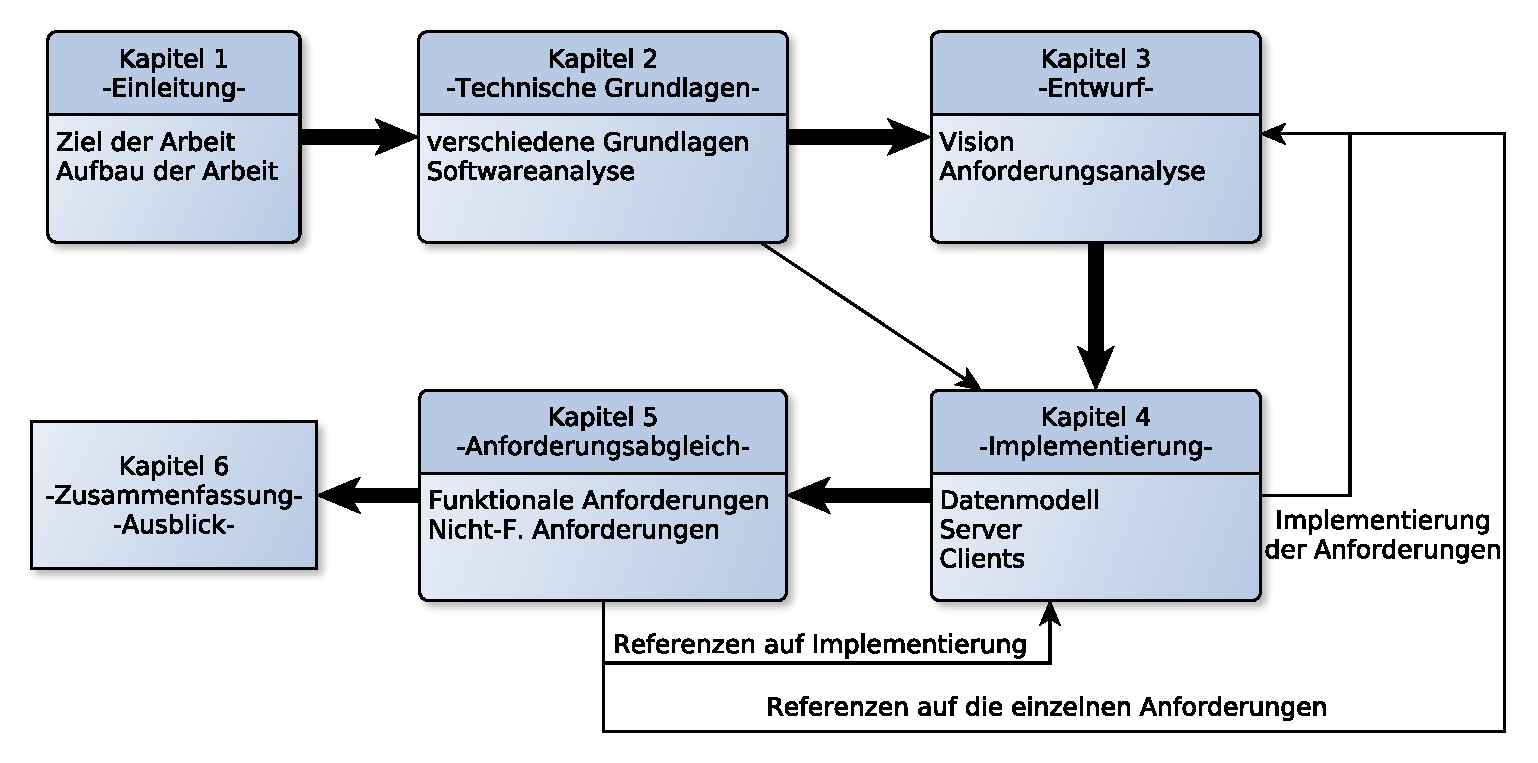
\includegraphics[scale=0.55]{images/AufbauDerArbeit}
	\caption[Aufbau der Arbeit]{Aufbau der Arbeit}
	\label{AufbauDerArbeit}
\end{figure}
Nach dieser Einleitung in das Thema wird im nächsten Kapitel auf die \textbf{technischen Grundlagen} der Arbeit eingegangen. Dieses Kapitel gibt zum einen Grundlagenwissen welches zum besseren Verständnis der Arbeit, insbesondere Kapitel Implementierung, beitragen soll und zum anderen wird eine \textbf{Software/Technologie Analyse} durchgeführt welche sich vorwiegend mit dem Thema Cross-Plattform-Entwicklung für mobile Endgeräte befasst.

Im darauf folgenden Kapitel "< \textbf{Entwurf} "> wird zuerst die \textbf{Vision} der Arbeit vorgestellt, welche darüber Aufschluss gibt, was genau von der entwickelten Plattform erwartet wurde und wie die Mechanismen von statten gehen sollten. Anschließend werden diese Erwartungen im Unterkapitel [\ref{Anforderungsanalyse}] \textbf{Anforderungsanalyse} in \textbf{Anforderungen} umgesetzt. 

In Kapitel \ref{_Implementierung} wird im Detail erklärt auf welche Weise diese \textbf{Anforderungen} umgesetzt sind. Zuerst wird das zugrundeliegende \textbf{Datenmodell} beschrieben. Anschließend werden die \textbf{Implementierungen} von \textbf{Server} und den beiden \textbf{Clients} näher beschrieben.

Im Verlauf von Kapitel \ref{Anforderungsabgleich} werden die \textbf{Anforderungen} aus Kapitel \ref{Anforderungsanalyse} im einzelnen betrachtet und gezeigt ob diese im Laufe der Arbeit erfüllt wurden. Hierbei werden Querverweise zu Kapitel \ref{_Implementierung} hergestellt um es dem Leser einfacher zu machen die zugrundeliegende \textbf{Implementierung} der \textbf{Anforderungen} zu finden.

Im letzten Kapitel wird eine Zusammenfassung sowie ein Ausblick über eine mögliche Weiterführung der Arbeit gegeben.



\chapter{Technologische Grundlagen} \label{Theoretische Grundlagen}
Im diesem Kapitel werden die Theoretischen Grundlagen der verwendeten Technologien im einzelnen betrachtet.
\todo{Leser klar machen warum die einzelnen dinge beschrieben werden}
\todo{mehr Bilder zur erklärung, auchmit bezug auf die arbeit}
\section{HTML 5}
In dieser Sektion wird nicht auf HTML5 allgemein eingegangen, es werden ausschließlich die Elemente erläutert welche verwendet wurden und durch die momentan neuste Spezifikation der Hypertext Markup Language spezifiziert sind. Ganz allgemein ist zu sagen, dass es HTML5 erlaubt interaktivere Anwendungen zu gestalten. HTML ist dabei die Sprache die verwendet wird, um das Aussehen der Seite zu spezifizieren. In der entwickelten Anwendung wurde sie in der Webanwendung des Therapeuten und auch in der Mobilen App für den Patienten verwendet.

Das \textbf{nav} Element wurde in der Therapeuten Webanwendung verwendet um die Navigationsleiste zu spezifizieren. Hier sind nur die Links zu den einzelnen Hauptseiten definiert. Durch die in den meisten Browsern automatisch verwendete CSS Eingenschaft \textit{display : block} wird diese als Box über die gesamte breite der Seite angezeigt \cite{SELFHTMLD16}. Durch Twitter Bootstrap bekommt die Navigationsleiste ihr aussehen und weitere Funktionalität.

Bei den verschiedenen \textbf{input} Elementen in beiden Clients konnte mittels HTML5 spezifiziert werden welche Art von Eingabe in dem jeweiligen Textfeld erwartet wird. Dies wurde verwendet um die Eingabe des Geburtsdatums des Patienten mit Hilfe des Input-Typs \textbf{date} zu erleichtern. Mittels des Input-Typs \textbf{email} wird automatisch kontrolliert ob die eingegebene E-Mail Adresse dem Standard für diese entspricht.

\section{Daten beim Aufrufen oder wechseln einer Seite übergeben}
Bei Webanwendungen wie die im Rahmen dieser Arbeit entstandenen, ist es immer wieder nötig, zum Beispiel beim Wechsel zu einer anderen Seite Daten an diese zu übergeben. Dies kann auf verschiedenen Wegen geschehen.

Bei kleiner Datenmengen wie Beispielsweise einer Id wird diese meinst in der URL übergeben. Diese wird dann an die eigentlich aufzurufende URL (z.B. http://eine.ip/index.html) nach einem \textbf{?} angehängt.
Die aufzurufende URL hat dann Beispielsweise die Form \\ \textit{http://eine.ip/index.html?patientId=eine1Id}.
Wird die Seite auf diese Art aufgerufen kann die Variable patientId dann von dieser ausgelesen werden. Soll mehr wie eine Variable übergeben werden,können diese mit dem \textbf{\&} Zeichen an einander angehängt werden.

Wenn größere Datenmengen zu übertragen sind, werden diese innerhalb des HTTP Objektes in dessen Rumpf übergeben. Dies wird in dieser Anwendung Beispielsweise verwendet, wenn nach der Anfrage an den Datenbank Server dessen Antwort mit dem Objekt im JSON Format Beispielsweise eines Patienten zurück gesendet wird.

 Angular, Mongoose MongoDB
 Client Webanwendungen, single page application Bootstrap
 Zentralisierung der Daten (Sicherheit)
 
 Android debug bridge ADB
 
\section{REST-Service}
Um eine gemeinsame Datenbasis zwischen den beiden Clients für Therapeut und Patient zu schaffen bietet der im Rahmen dieser Arbeit entwickelte Server einen REST-Service zum abrufen der in der Datenbank gespeicherten Daten an. Mit dessen Hilfe können die Daten zu den Patienten, Aufgaben und Fragebögen über das Internet mittels HTTP Anfragen auf jedem Gerät abgerufen und verändert werden. Das Programmierparadigma eines REST-Services soll dabei verschiedenen Prinzipien folgen.

Zum einen soll dieser Service \textbf{Zustandslos} sein. Bei jedem Aufruf müssen somit alle zum verstehen der Nachricht nötigen Daten übermittelt werden.
Ein weiteres Prinzip ist die \textbf{Adressierbarkeit} der einzelnen Ressourcen, welches in dieser Anwendung durch die einzigartige Id jedes Objekts realisiert wurde.
\subsection{Die HTTP-Methoden}
Um mit dem Service zu interagieren stehen verschiedene HTTP-Methoden zu Verfügung. Welche hier kurz erklärt werden.
\paragraph{HTTP-GET}
Mittels HTTP-GET wird dem Server signalisiert, dass Daten abgerufen werden wollen. Hierbei kann eine allgemeine Anfrage gestellt werden um alle vorhandenen Daten zu erhalten oder mittels der unter Adressierbarkeit angesprochen Id ein bestimmtes Objekt angefordert werden.
\paragraph{HTTP-POST}
Diese Methode wird verwendet um ein neues Objekt in der Datenbank anzulegen. Der Server antwortet hierbei mit dem Angelegten Objekt welches die vom Server erzeugte, einzigartige Id enthält.
\paragraph{HTTP-PUT}
Mit Hilfe der PUT-Methode kann ein auf dem Server vorhandenes Objekt verändert werden, hierbei muss die Id bekannt sein und übermittelt werden.
\paragraph{HTTP-DELETE}
Durch diese Methode kann ein Objekt anhand seiner Id auf dem Server gelöscht werden.

\section{Sicherheit}
Da es sich bei den ausgetauschen Daten um prisante Patientendaten handelt sollte das Thema Sicherheit sehr groß geschrieben werden. Da es jedoch den Rahmen dieser Arbeit überzogen hätte, wird es nur theoretisch betrachtet und wurde während der Implementierung völlig außer Acht gelassen. Bevor die Plattform mit realen Daten verwendet wird muss in jedem Fall zuerst verhindert werden, dass unbefugte auf die Daten der Patienten zugreifen können. In diesem Abschnitt sollen Ideen und Anregungen gegeben werden wie dies bewerkstelligt werden kann. 
Da in einem REST-Service nicht von Haus aus Schutzmechanismen eingebaut sind liegt es in der Hand des Entwicklers die oben beschriebenen, unsicheren HTTP Methoden vor dem Zugriff durch unberechtigte zu schützen.
\subsection{SSL}

\subsection{OAuth}

\section{BPMN-IO}

\subsection{Aufbau der exportierten XML Datei}
 
 

\section{Anwendungsentwicklung} \todo{bezug auf die Anwedung}
Am Anfang jeder mobilen Anwendung steht die Entscheidung auf welchen Geräten diese laufen soll. Natürlich besteht die Möglichkeit eine Anwendung nativ für eine bestimmte Plattform zu entwickeln.

Um die Anwendung auf anderen Plattformen zu bringen ist es dann jedoch nötig diese praktisch neu für diese zu implementieren. Aus diesem Dilemma heraus entstanden verschiedenen Frameworks die es dem Entwickler möglich machen, direkt für mehrere Plattformen zu entwickeln. Hierdurch ist es dann möglich seinen Code nur einmal zu schreiben und diesen dann direkt, mithilfe eines Frameworks, wie zum Beispiel eines Browsers auf den verschiedene Plattformen laufen zu lassen.

Es müssen dann nur einige wenige Abschnitte des Codes nativ für die jeweilige Plattform geschrieben werden, wenn diese nicht verallgemeinerbar sind bzw. nicht schon durch eine Bibliothek vereinheitlicht wurden. Ein Beispiel wäre hier der Zugriff auf Dateien, hier ist es nicht möglich den Zugriff direkt zu verallgemeinern, da die verschiedenen Betriebssysteme unterschiedliche Dateisysteme Verwenden.

Eine der Grundvoraussetzungen dieser Arbeit sollte die Verfügbarkeit für möglichst viele Patienten sein. Aus diesem Grund wurde vorab untersucht durch welche Techniken es möglich ist, die Hürde der vielen verschiedenen Endgeräte und damit verbundenen Betriebssysteme umgehen zu können. Durch die enge Bindung der Therapeutensoftware an den Server viel die Wahl von vorn herein auf eine sogenannte \textbf{Single-Page-Application} in Form einer Website.


\subsection{Anwendungsentwicklung für mobile Geräte}
Das größte Problem der Anwendungsentwicklung für Smartphones ist, dass es viele verschiedene mobile Betriebssystemen gibt. Ein kleiner Trost für jeden Entwickler ist dabei, dass sich der Hauptteil der Nutzer auf einige wenige Plattformen beschränkt. Mit einer Anwendung für Android, IOS und Windows kann man somit den größten Teil der Nutzer erreichen. Diese decken über 99\% \cite{STA2016} der der Smartphone Benutzer ab.



PhoneGap + Ionic[1 und 2 ] %http://ionicframework.com/docs/overview/#cordova
"What the ionic framework provides is the native look and feel and the user interface interactions"
\subsubsection{Ionic - Cordova}
\todo{package.json erklären}
\paragraph{Proxys zum Debuggen im Browser - Das CORS-Problem}

\subsubsection{Xamarin}

(http://thinkapps.com/blog/development/develop-for-ios-v-android-cross-platform-tools/) 

 
\subsubsection{Plattform spezifische Entwicklung}
Durch die nativen Anwendungsentwicklung wird eine mobile Anwendung nur jeweils für eine Plattform entwickelt. Hierdurch hat man aber den Vorteil, dass man durch wegfallen jegliches Frameworks die maximale Geschwindigkeit und minimale Reaktionszeiten erzielt.

Dies ist vor allem wichtig bei Rechenintensiven Anwendungen wie Spielen oder ähnlichem. Des weiteren hat man durch die native Entwicklung den vollen Zugriff auf jegliche im Smartphone verbaute Hardware und Betriebssystem Features. Bei Verwendung eines Frameworks müssen hier oft Abstriche gemacht werden.
\todo{die entwicklung für die einzelnen Plattformen aufzeigen}
\subsubsection{Cross Plattform Entwicklung}
Von Cross Plattform Entwicklung spricht man, wenn der Code der entwickelten Anwendung nicht nur für eine spezifische Plattform verwendbar ist. Durch verschiedene Frameworks ist es möglich, dass der Entwickler die Anwendung nur ein mal schreib und diese dann auf den meist verwendeten Betriebssystemen läuft oder für diese Übersetzt wird. Dies wird Grundlegend auf \textbf{3 verschiedenen} Wegen erreicht:

\paragraph{Web-Apps / Webanwendungen}laufen im, vom Betriebssystem zur Verfügung gestellten Webbrowser. Hierbei ist das Betriebssystem völlig egal, es werden nur einige Voraussetzungen an den Webbrowser gestellt, welche jedoch von dem meisten neuer Browsern erfüllt werden.

Ebenso wird eine aktive Internetverbindung benötigt wenn die App ausschließlich online zur Verfügung steht. Um dies zu umgehen wurde in HTML5 verschiedenen Möglichkeiten eingebaut um Code und Daten lokal zwischenzuspeichern zu können. Dies bietet den Vorteil, dass die App schnell veröffentlicht und aktualisiert werden kann. Wenn der Nutzer die Anwendung mit einer aktiven Internet Verbindung öffnet, aktualisiert sich die App automatisch. 

Der Nachteil dadurch das die App im Webbrowser läuft ist, dass man nur Zugriff auf die Funktionen hat, die der verwendete Browser bietet. Da ein Webbrowser nicht zwangsläufig auf einem mobilen Gerät mit diversen Sensoren laufen muss, ist der Zugriff auf die gängigen Sensoren in einem mobilen Endgerät meinst sehr eingeschränkt. Auf Grund dessen muss man sich bei der Web-App Entwicklung meist auf Kamera, Datenpersistenz und GPS beschränken.

Durch die Zentralisierung der App sieht diese auf jedem Gerät gleich aus. Dies erscheint im ersten Augenblick positiv, der Benutzer jedoch ist an das Bedienkonzept seines Betriebssystems gewohnt, wodurch Apps welche nicht auf das Betriebssystem zugeschnitten sind meist keinen sehr großen Anklang bei den Nutzern findet. 

\todo{inhalt des links mit reinbringen. link im kommentar}%https://de.wikipedia.org/wiki/Webanwendung#/media/File:Webanwendung_client_server_01.png

\paragraph{Hybride Apps}\label{Hybride Apps} basieren wie auch die Web-Apps auf den Webtechnologien HTML5, CSS und JavaScript. Laufen aber im Gegensatz zu dem Web-Apps in einem mitgelieferten Minibrowser(Webview Container).

Dieser Container ist in einer nativen App eingebettet was den Zugriff auf die System APIs des Geräts erlaubt. Durch das einbetten von nativen Code ist der Zugriff auf alle vom Betriebssystem zur Verfügung gestellten Funktionen möglich. wie z.b. GPS, Kamera, Betriebssystem Benachrichtigungen und die verschiedenen Sensoren(Beschleunigung, Umgebungslicht, Hall, Gyroskop,...). 

Da die Anwendung im Herzen eine Internetseite ist, ist es implizit möglich diese unter einer URL zu veröffentlichen und wie eine Web-App zu behandeln. Dann jedoch auch mit den Einschränkungen die diese bietet.

Für den Entwickler sehr angenehm sind oft angebotene "Live-View" Technologien. Diese erlauben durch speichern einer HTML oder JavaScript Projektdatei ein neu laden der App im Webbrowser zu initiieren. Dies bietet ein schnelles Designen der Oberfläche und implementieren grundlegender Funktionen. System eigene Funktionen müssen jedoch auf einem Gerät oder im Emulator getestet werden. Hierzu ist dann compilieren, packen und ausliefern notwendig, was etwas Zeit benötigt.

Ionic machts für jedes Gerät individuell.....

\todo{Wikipediaartikel is nochmal anders beschrieben} %https://de.wikipedia.org/wiki/Mobile_App#Hybrid-Apps

\paragraph{Native Cross Plattform Apps} mit gemeinsamer Codebasis verspricht \textbf{Xamarin}, ein Projekt das auf der quellen-offenen Implementierung von Microsofts .NET Framework, Mono basiert \cite{MONO16}. Mittels des Mono Frameworks ist es möglich C\# Code auf verschiedenen Betriebssystemen laufen zu lassen. Der geschriebene Code wird dann beim Bauvorgang der App in Nativen Code umgesetzt. Es fällt somit im Gegensatz zu den Hybriden Apps, das Framework auf dem Endgerät weg, wodurch Rechenkapazität gespart wird. Was diese Plattform vor allem für rechenintensive Anwendungen interessant macht.

Bei der Erstellung einer Cross Plattform App mittels Xamarin muss man zuerst festlegen, auf welchen Betriebssystemen diese später laufen soll. Aus dieser Auswahl wird eine Schnittmenge der Funktionen gebildet die zur Verfügung stehen und eine sogenannte \textbf{Portable Class Library} erzeugt. Diese fungiert dann als einheitliche Schnittstelle bei Api aufrufen an das Betriebssystem.

Es sind jedoch nur die Funktionen Plattform-übergreifend nutzbar, welche von allen ausgewählten Betriebssystemen angeboten werden und von Mono implementiert sind. 
Sollte der Entwickler Zugriff auf System-eigene Funktionen benötigen, welche nicht von Mono abgedeckt werden, hat er mit Xamarin.iOS und Xamarin.Android die Möglichkeit alle System-eigenen Funktionen verwenden zu können. Zur Vereinheitlichung unter einer gemeinsamen GUI ist es dann aber nötig die Funktion für jedes Betriebssystem separat zu entwickeln und zu pflegen.

Mittels Xamarin.Forms ist es möglich die GUI der App Plattform-übergreifend zu gestalten. Hierzu wird die Oberfläche mittels einer eigenen, XML ähnlichen, Sprache namens \textbf{Extensible Application Markup Language (kurz XAML)} beschrieben. Die so spezifizierten Views werden dann auf die einzelnen Betriebssysteme zugeschnitten, um dem Anwender eine gewohnte Umgebung zu bieten. 

\section{Software Analyse}



\chapter{Implementierung}\label{Implementierung}
\section{Entwurf}
\subsection{Anforderungsanalyse}

\subsection{Architekturentwurf}

\section{Implementierung}

\subsection{Therapeuten Client}

\subsection{Patienten App}

\chapter{Anforderungsabgleich} \label{Anforderungsabgleich} \todo{Anforderungstabellen mit erwähnen, wo kommen die Anforderungen her}
Im folgenden Kapitel wird ein Anforderungsabgleich vorgenommen, dieser gibt Aufschluss darüber welcher der in Kapitel Anforderungsanalyse \ref{Anforderungsanalyse} spezifizierten Anforderungen schlussendlich implementiert wurden.
Hierbei wird im einzelnen auf die jeweiligen Anforderungen eingegangen und Querverweise in das Kapitel Implementierung \ref{_Implementierung} hergestellt. Um die Reihenfolge von Kapitel \ref{Anforderungsanalyse} beizubehalten wird mit den Funktionalen Anforderungen begonnen, anschließend werden die Nicht-Funktionalen Anforderungen untersucht.
\section{Funktionale Anforderungen}
In diesem Kapitel werden die funktionalen Anforderungen untersucht. Sowohl an den Datenbank Server sowie für die beiden Clients.
\subsection{Datenbank Server}
Im folgenden Abschnitt werden die Anforderungen an den Datenbank Server aus Tabelle \ref{NichtFunktionaleAnforderungenServer} untersucht.
\paragraph{Anforderung 1.1 - Datenpersistenz  \textcolor{green}{\checkmark}}
 wurde wie in Kapitel \ref{_ImpDatenbankServer} beschreiben umgesetzt. Für die Datenpersistenz wurde eine MongoDB Datenbank auf dem Server installiert, diese legt ihr Daten für den Nutzer nicht sichtbar auf dem Dateisystem ab, wo diese persistent gespeichert werden.

\paragraph{Anforderung 1.2 - Daten Sicherung  \textcolor{red}{X}}
Dieses Feature wurde nicht Implementiert. Da bisher nicht mit realen Daten bearbeitet wurde war auch eine Sicherung dieser nicht nötig.

\paragraph{Anforderung 1.3 - Datenschnittstelle \textcolor{green}{\checkmark}}
Wie in Kapitel \ref{_ImpDatenbankServer} beschreiben, wurde mit Hilfe des express Frameworks eine REST-API implementiert welche HTTP anfragen entgegen nimmt. Hierdurch ist es Möglich, Daten aus der Datenbank anzufragen, zu verändern bzw. löschen so wie neue Datensätze anzulegen.


\subsection{Therapeuten Client}
Die Anforderungen an den Therapeuten Client \textbf{wurden alle erfüllt.}
\paragraph{Anforderung 2.1 - Patientenverwaltung \textcolor{green}{\checkmark}}
Dieses Feature \textbf{wurde Implementiert} indem dem Therapeuten Client wie in Kapitel \ref{_ImpTCPatientUebersicht} beschreiben, eine Seite hinzugefügt wurde auf derer er eine Übersicht über seine Patienten hat. Hier können Patienten auch gelöscht werden - Anforderung 2.1.3.

Zusätzlich wurde wie in Kapitel \ref{_ImpTCPatientDetail} beschreiben eine Seite erzeugt mit welche der Therapeut Patienten anlegen bzw. editieren kann - Anforderungen 2.1.1 und 2.1.2.

\paragraph{Anforderung 2.2 - Aufgabenverwaltung \textcolor{green}{\checkmark}}
Mittels der in Kapitel \ref{_ImpTCAufgaben} beschriebenen Seiten ist es dem Therapeuten möglich die Vorlagen für Aufgaben / Übungen zu verwalten. Wie bei der Patientenverwaltung gibt es eine Übersicht in welcher einzelne Aufgaben ausgewählt oder gelöscht (Anforderung 2.2.3) werden können. Mittels der ebenso in Kapitel \ref{_ImpTCAufgaben} beschriebenen Seite zum anlegen und editieren von Aufgaben werden den Anforderungen 2.2.1 und 2.2.2 abgedeckt.

\paragraph{Anforderung 2.3 - Fragebogenverwaltung \textcolor{green}{\checkmark}}
Wie für die Verwaltung von Patienten und Aufgaben/Übungen wurde auch für die Fragebogenverwaltung eine eigene Seite Implementiert, welche in Kapitel \ref{_ImpTCFragebogen} beschreiben wird. Diese bietet die Möglichkeit Fragebögen zu löschen(Anforderung 2.3.3). Die ebenfalls in Kapitel \ref{_ImpTCFragebogen} beschriebene Seite zum erstellen und editieren von Fragebögen erfüllt die Anforderungen 2.3.1 und 2.3.2.

\subsection{Aufgaben-/Übungsvorlagen}
Die Anforderungen an die Aufgaben-/Übungsvorlagen wurden, wie in Tabelle \ref{TabelleAnforderungsabgleichVorlagen} beschrieben, Teilweise erfüllt.
A.1 bis A.3 sowie A.6 wurden wie in Kapitel \ref{_ImpTCAufgaben} beschreiben erfüllt. 

\begin{table}[htbp]
	\begin{center}
		\begin{tabular}{p{0,5cm} p{6,5cm} p{7,5cm}}
			\rowcolor{black!20} \textbf{Nr.} & \textbf{Bezeichnung} & \textbf{Erfüllt?} \\ \toprule 
			A.1 & \textbf{Name} & \textcolor{green}{\checkmark} \\ \hline \addlinespace
			A.2 & \textbf{Beschreibung} & \textcolor{green}{\checkmark} \\ \hline \addlinespace
			A.3 & \textbf{Materialien} & \textcolor{green}{\checkmark} \\ \hline \addlinespace
			A.4 & \textbf{Kontrollmechanismen} & \textcolor{red}{X} \\ \hline \addlinespace
			A.5 & \textbf{Kategorisierung} & \textcolor{red}{X}  \\ \hline \addlinespace
			A.6 & \textbf{Verschiedene Erledigungskontexte} & Es wurde nur der Zeitkontext implementiert \\ \hline \addlinespace
		\end{tabular}
	\end{center}
	\caption[Anforderungsabgleich der Aufgaben-/Übungsvorlagen]{Anforderungsabgleich der Aufgaben-/Übungsvorlagen}
	\label{TabelleAnforderungsabgleichVorlagen}
\end{table}

\subsection{Fragebögen}
Die in Tabelle \ref{TabelleFunktionaleAnforderungenFragebogen} gezeigten Anforderungen wurden abgesehen von Anforderung B.2 \textbf{erfüllt}. Anforderung B.2 wurde als nicht mehr wichtig erachtet, da der Name ausreicht, um einen Fragebogen zu identifizieren. Durch die grafische Darstellen mittels des in Kapitel \ref{_ImpTCFragebogen} beschrieben Tools zur Erstellung/Bearbeitung von Fragebögen wird das wiederfinden eines bestimmten Fragebogens weiter vereinfacht.

\textbf{Anforderung B.3} wurde erfüllt, indem es mittels des grafischen Tools möglich ist, die Fragen und Antworten nach belieben mit einander zu verbinden. Hierdurch kann der Therapeut frei wählen, welche Frage auf eine gegebene Antwort folgt.

Verschiedene Antwortmöglichkeiten wie in \textbf{Anforderung B.4} gefordert wurden wie in Kapitel \ref{_ImpTCFragebogen} beschreiben mit Hilfe eines Zusatz Panels realisiert. Da dies aber nicht sehr intuitiv ist, sollte hier die Möglichkeit wahrgenommen werden, dass man in dem verwendeten Tool neue Elemente einbauen kann. Hierdurch wäre es Beispielsweise möglich zusätzliche Elemente für die einzelnen Fragetypen zu Verfügung zu stellen. Da in dem Tool auch auf Klicks reagiert werden kann, wäre zur Vereinfachung dieses Vorgangs auch ein Kontextmenü denkbar, in welchem man einem allgemeinen Frageelement einen Typ zuweisen kann.

\paragraph{Fragetypen}
Wie in der Tabelle \ref{FrageTypen} im Kapitel \ref{_ImpTCFragebogen} zu sehen wurden die Anforderungen C.1 bis C.4 in vier verschiedenen Typen von Fragen realisiert.


\begin{description}
	\item[Anforderung C.1 (Einzelantwort)]\hfill \\
	 wurde als Typ \textbf{single} spezifiziert.
	\item[Anforderung C.2 (Mehrfachantwort)] \hfill \\
	 wurde als Typ \textbf{multi} spezifiziert.
	\item[Anforderung C.3 (Bewertung)]\hfill \\
	wurde als Typ \textbf{text} bewertet.
	\item[Anforderung C.4 (Freitext)]\hfill \\
	wurde als Typ \textbf{rating} spezifiziert.
\end{description}

\subsection{Patienten Client}
Die Anforderungen 3.1 bis 3.7 aus Tabelle \ref{TabelleFunktionaleAnforderungenTherapeutClient}  wurden wie in Kapitel \ref{_ImpPatientClient} beschrieben implementiert. Ein Überblick über die einzelnen Anforderungen mit Querverweisen in das Implementierungskapitel sind in Tabelle \ref{TabelleAnforderungsabgleichPatientClient} zu finden.

\begin{table}[H]
	\begin{center}
		\begin{tabular}{p{0,5cm} p{4cm} p{2cm} p{2,5cm}}
			\rowcolor{black!20} \textbf{Nr.} & \textbf{Anforderung} & \textbf{Erfüllt?} & \textbf{Beschreibung} \\	\toprule
			3.1 & User Identifikation & \textcolor{green}{\checkmark} & \ref{_ImpPatientClient} \\ \hline \addlinespace
			3.2 & Aufgabenanzeige & \textcolor{green}{\checkmark} & \ref{_ImpPCAufgaben} \\ \hline \addlinespace
			3.3 & Detailanzeige der Aufgabe  & \textcolor{green}{\checkmark} & \ref{_ImpPCAufgabenDetail} \\ \hline \addlinespace
			3.4 &Anzeige der Materialien & \textcolor{green}{\checkmark} & \ref{_ImpPCAufgabenDetail} \\ \hline \addlinespace
			3.5 &Verändern des Erledigungskontext & \textcolor{green}{\checkmark} & \ref{_ImpPCAufgabenDetail} \\ \hline \addlinespace
			3.6 &Erinnerung & \textcolor{green}{\checkmark} & \ref{_ImpPCErinnerungen} \\ \hline \addlinespace
			3.7 &Fragebogen beantworten & \textcolor{green}{\checkmark} & \ref{_ImpPCFragebogen} \\ \hline \addlinespace
		\end{tabular}
	\end{center}
	\caption[Anforderungsabgleich des Patienten Clients]{Anforderungsabgleich des Patienten Clients}
	\label{TabelleAnforderungsabgleichPatientClient}
\end{table} 

\section{Nicht-funktionale Anforderungen}
Im folgen Kapitel werden die nicht-funktionalen Anforderungen beleuchtet. 
\subsection{Datenbank Server}
Die nicht-funktionalen-Anforderungen des Datenbank Servers welche in Tabelle \ref{NichtFunktionaleAnforderungenServer} aufgezeigt sind, werden im folgenden Abschnitt untersucht.
\paragraph{Anforderung 4.1 - kurze Reaktionszeiten  \textcolor{green}{\checkmark}} Da der Server auf erprobten Technologien wie NodeJS und dem Express Framework beruht. Kann davon aus gegangen werden das diese auch für größere Nutzerzahlen geeignet sind. In der erstellten Testumgebung ist die Reaktionszeit der Anwendung nie negativ aufgefallen.
\paragraph{Anforderung 4.2 - Sicherheit  \textcolor{red}{X}} Da die Plattform bisher nicht mit realen Patientendaten verwendet wurde, war keine Notwendigkeit diese zu verschlüsseln. Bevor die Plattform mit realen Daten verwendet wird, müssen diese vorher vor dem Zugriff unbefugter geschützt werden. Hierzu sind im Kapitel \ref{_GrundlagenSicherheit} Anregungen gegeben.

\subsection{Therapeuten / Patienten Client}
Im folgen Absatz werden die in Tabelle \ref{NichtFunktionaleAnforderungenClients} spezifizierten, nicht-funktionalen Anforderungen an die beiden Clients untersucht.
\paragraph{Anforderung 5.1 - Natives Design \textcolor{green}{\checkmark}} Da der \textbf{Therapeuten Client} in Form einer Website implementiert wurde, kann es für diesen kein Natives Design geben. Dieser hat dann aber den Vorteil, dass er auf jedem Gerät gleich aussieht. Einzig bei mobile Endgeräte, gemessen an der Displaygröße, wird das User-Interface der Anwendung angeglichen um kleinen Displays gerecht zu werden. Darauf, welches Betriebssystem zugrunde liegt wird nicht reagiert.

Das native Design des \textbf{Patienten Clients} wurde durch die Verwendung von Ionic weitgehendst umgesetzt. Die wichtigsten Bedienelemente werden durch Ionic an das jeweilige Betriebssystem angeglichen. Man sieht jedoch schon noch, dass die App im Herzen eine Website ist. Durch eine Überarbeitung des User-Interfaces kann das native Feeling der App extrem erhöht werden.

\paragraph{Anforderung 5.2 - vertretbare Reaktionszeiten \textcolor{green}{\checkmark}} Da für beide Clients sehr erprobte Technologien verwendet wurden und die Anwendungen auch keine großen Rechenleistungen benötigen wurde keine Untersuchungen zu den Reaktionszeiten vorgenommen. Während der Verwendung der Testumgebungen sind auch hier keine unzumutbaren Verzögerungen aufgefallen.



\chapter{Zusammenfassung und Ausblick} \label{Zusammenfassung und Ausblick}
\subsection{Zusammenfassung}
\subsection{Ausblick}

\appendix
% hier Anhänge einbinden
%\input{chapters/AVerwendungDesModems}

\backmatter

\bibliographystyle{plaindin} % Nummern und alphabetisch sortiert
%\bibliographystyle{alphadin} % Buchstaben und sortiert
%\bibliographystyle{abbrvdin} % Nummern und abgekürzte Namen
%\bibliographystyle{unsrtdin} % Nummern und unsortiert
\addcontentsline{toc}{chapter}{Literaturverzeichnis}
\bibliography{2011_Dipl_utf8}
\nocite{*}
\listoffigures
\listoftables
\clearpage
\thispagestyle{empty}

Name: \fullname \hfill Matrikelnummer: \matnr \vspace{2cm}

\minisec{Erklärung}

Ich erkläre, dass ich die Arbeit selbständig verfasst und keine anderen als die angegebenen Quellen und Hilfsmittel verwendet habe.

Außerdem erkenne ich die Satzung der Universität Ulm zur Sicherung guter wissenschaftlicher Praxis an.\vspace{2cm}

Ulm, den \dotfill

\hspace{10cm} {\footnotesize \fullname}
\end{document}
\grid
